\documentclass[conference]{IEEEtran}
\usepackage{cite}
% *** GRAPHICS RELATED PACKAGES ***
%
\ifCLASSINFOpdf
  % \usepackage[pdftex]{graphicx}
  % declare the path(s) where your graphic files are
  % \graphicspath{{../pdf/}{../jpeg/}}
  % and their extensions so you won't have to specify these with
  % every instance of \includegraphics
  % \DeclareGraphicsExtensions{.pdf,.jpeg,.png}
\else
  % or other class option (dvipsone, dvipdf, if not using dvips). graphicx
  % will default to the driver specified in the system graphics.cfg if no
  % driver is specified.
  % \usepackage[dvips]{graphicx}
  % declare the path(s) where your graphic files are
  % \graphicspath{{../eps/}}
  % and their extensions so you won't have to specify these with
  % every instance of \includegraphics
  % \DeclareGraphicsExtensions{.eps}
\fi
\usepackage[linesnumbered,vlined]{algorithm2e}
\usepackage[ansinew]{inputenc}
\usepackage{epsfig}
\usepackage{amsfonts}
\usepackage{amssymb}
\usepackage{subfigure}
\usepackage[usenames]{color}
\usepackage{soul}
\usepackage{comment}
\usepackage{multirow}
\usepackage[cmex10]{amsmath}
\usepackage{bm}
\usepackage{setspace}

% correct bad hyphenation here
\hyphenation{op-tical net-works semi-conduc-tor}

\newcommand{\Az}[1]{{\bf{#1}}}


\begin{document}
\title{Future Evolution of CSMA Protocols for the IEEE 802.11 Standard}


% author names and affiliations
% use a multiple column layout for up to three different
% affiliations
\author{\IEEEauthorblockN{Luis Sanabria-Russo, Azadeh Faridi, Boris Bellalta, Jaume Barcelo, Miquel Oliver}
\IEEEauthorblockA{
Universitat Pompeu Fabra\\
Roc Boronat 183, 08018 Barcelona\\
Email: \{name.surname@upf.edu\}}
}

% use for special paper notices
%\IEEEspecialpapernotice{(Invited Paper)}




% make the title area
\maketitle


\begin{abstract}
%\boldmath
In this paper we present the requirements of candidate protocols to replace the prevalent CSMA/CA medium access control.
We discuss the possibility of further preventing collisions and provide an overview of the related work.
We specify a protocol that is a candidate for replacing CSMA/CA in pseudocode and use simulation to assess performance metrics such as throughput, fairness and collision probability.
\end{abstract}


% For peer review papers, you can put extra information on the cover
% page as needed:
% \ifCLASSOPTIONpeerreview
% \begin{center} \bfseries EDICS Category: 3-BBND \end{center}
% \fi
%
% For peerreview papers, this IEEEtran command inserts a page break and
% creates the second title. It will be ignored for other modes.
\IEEEpeerreviewmaketitle



\section{Introduction}
% no \IEEEPARstart
% You must have at least 2 lines in the paragraph with the drop letter
% (should never be an issue)

Since the popularization of the IEEE 802.11 standard, several works \cite{bharghavan1994map,wang2004ncr,cali2000dti,lopez-toledo2006aoi,
barcelo2008lba,bellalta2009vtc,he2009srb,barcelo2010fcc,fang2011dlm,hui2011epp,barcelo2011tcf} \Az{(missing any?)} have proposed modifications to CSMA/CA (Carrier Sense Multiple Access with Collision Avoidance), the contention protocol used in the standard for sharing the medium. \Az{Despite the throughput improvement offered by all these works, none of the proposed modifications have yet been adapted by the standard.}

It is essential for a candidate CSMA/CA replacement to
\begin{itemize}
  \item provide performance advantages in terms of throughput and/or short term fairness;
  \item be backward compatible with the current implementation;
  \item support a large number of simultaneous contenders; and 
  \item be a simple evolution, in terms of implementation, to ease the transition and reduce the time to market (optional but desirable).
\end{itemize}

The aforementioned works can be categorized in three groups regarding the approach they use. \Az{In this paper, we will focus on the last of these three groups, proposing an additional enhancement to make it more adaptable to network size variations, and make the case for its adaptation by the standard.}

In the first group, represented by \cite{bharghavan1994map,wang2004ncr}, a throughput increase is obtained in saturation conditions by preventing the contention window from resetting to its minimum value after each successful transmission. However this performance gain comes at the expense of reduced short term fairness, since nodes that have recently gone through a sequence of consecutive collisions are forced to stay at a higher back-off stage and thus are further penalized by less frequent transmissions.

In the second group of works, exemplified here by \cite{cali2000dti,lopez-toledo2006aoi}, an accurate estimate of the number of contenders is used to adjust the contention parameters. This approach offers some throughput and fairness gains, but at the expense of increased implementation complexity. In addition, as the number of contenders is estimated relying on the number of collisions, the presence of channel errors further complicates the estimation \Az{[Complicates, or renders it inaccurate? Is there a work-around offered?]}.
Furthermore, there is a fundamental trade-off between the stability and the speed of reaction of the estimation.

When it comes to backward compatibility, neither of the aforementioned solutions are able to fairly share the medium with legacy devices.
In fact, these proposals are, generally speaking, less aggressive than the currently implemented CSMA/CA protocol. Consequently, in a hypothetical mixed network in which the new and old protocols coexist, the new stations would receive a smaller share of the available bandwidth.

A more important limitation of the two approaches exposed so far is that the throughput is bounded by that of CSMA/CA with optimal configuration \cite{cali2000dti,bianchi2000pai}.

The third group of solutions, which is the focus of the current paper, can deliver a throughput above the maximum attainable by CSMA/CA. This performance boost is achieved mainly by the use of deterministic backoff after successful transmissions, which reduces the chances of collisions for nodes that were successful in their previous transmission. Furthermore, under certain conditions, a collision-free operation can be reached. \Az{We will refer hereafter to the class of algorithms that use deterministic backoffs after successful transmissions as CSMA with Enhanced Collision Avoidance (CSMA/ECA).} This approach was first introduced in \cite{barcelo2008lba} \Az{(Does this contain analysis?)}, and later a more detailed analysis for both saturated and non-saturated conditions was presented in \cite{bellalta2009vtc}.
A more in-depth study is carried out in \cite{he2009srb}, including realistic elements such as the possibility of Clear Channel Assessment errors.
Different aspects of fairness are addressed in \cite{he2009srb,barcelo2010fcc,fang2011dlm}.
The performance in realistic channels, taking into account the Auto Rate Fallback mechanism, is evaluated in \cite{martorell2012pec,martorell2012tfl}.

Even though initial research efforts where focused on the WLAN collision problem, more recent papers try to extend the idea to multi-hop networks.
In \cite{hui2011epp}, the multi-hop slotted case explored.
The more realistic situation in multi-hop networks in which the time is not slotted is studied in \cite{barcelo2013dcc}.

The same principles that we exploit to prevent collisions in WLANs can be used in other areas of radio resource management in wireless area networks \cite{duffy2011dcs,checco2012scs,checco2012lbc,khan2013aso}.

In all the previous work on collision-free operation in WLANs mentioned so far, there is the limitation that the number of contenders should not exceed the value of the deterministic backoff used after successful transmissions.
If this value is exceeded, it is no longer possible to achieve collision-free operation.
A first solution to solve this problem is presented in \cite{barcelo2011tcf}, but it requires the presence of a central entity (typically the access point) that instructs the other nodes to adjust the value of their deterministic backoff.

In the current paper, we present a completely distributed solution, called {\it backoff stage hysteresis} or simply hysteresis, to accommodate a large number of contenders in a fair collision-free fashion. We furthermore detail pseudo-code algorithms for three different types of CSMA/ECA and highlight how they can be easily implemented using simple modifications to the currently-used CSMA/CA algorithm. We will then present some performance evaluation, quantifying the performance gain that these three types of CSMA/ECA can achieve, both in terms of throughput and fairness.

\Az{-comment about backward compatibility and other items in the candidate requirements.}

\section{Enhanced CSMA/CA}

\begin{algorithm}
\While{the device is on}
{
  %\tcc{Initialize retransmission attempts.}
  $r \leftarrow 0$ ; $s \leftarrow 0$ \;
  %\tcc{Initialize backoff counter.}
  $b \leftarrow \mathcal{U}[0,2^s\rm{CW}_{min}-1]$\;
  \While{there is a packet to transmit}{
    %\tcc{Initialize $a$.}
    \Repeat{($r = R$) or (success)}{
      %\tcc{First, backoff.}
      \While{$b>0$}{
        wait 1 slot \;
        $b \leftarrow b-1$ \;
      }
      Attempt transmission of 1 packet \;
      \If{collision}{
        %\tcc{Random backoff.}
        $r \leftarrow r+1$ \;
        $s \leftarrow \min (s+1,S)$ \;
        $b \leftarrow \mathcal{U}[0, 2^s \rm{CW}_{min} -1]$\;
      }
    }
    \eIf{success}{
      %\tcc{Random backoff.}
      $r \leftarrow 0$ \;
      $s \leftarrow 0$ \;
      $b \leftarrow \mathcal{U}[0,2^{s}\rm{CW}_{min}-1]$\;
    }
    {
      Discard packet\;
      $r \leftarrow 0$ \;
      $s \leftarrow 0$ \;
      $b \leftarrow \mathcal{U}[0,2^s \rm{CW}_{min}-1]$\;
    }
  }
  Wait until there is a packet to transmit \;
}
\caption{CSMA/CA}
\label{alg:CSMA_CA}
\end{algorithm}


\begin{algorithm}
\While{the device is on}
{
  $r \leftarrow 0$ ; $s \leftarrow 0$ \;
  $b \leftarrow \mathcal{U}[0,2^s\rm{CW}_{min}-1]$\;
  \While{there is a packet to transmit}{
    %\tcc{Initialize $a$.}
    \Repeat{($r = R$) or (success)}{
      %\tcc{First, backoff.}
      \While{$b>0$}{
        wait 1 slot \;
        $b \leftarrow b-1$ \;
      }
      Attempt transmission of 1 packet \;
      \If{collision}
      {
        %\tcc{Random backoff.}
        $r \leftarrow r+1$ \;
        $s \leftarrow \min (s+1,S)$ \;
        $b \leftarrow \mathcal{U}[0, 2^s  \rm{CW}_{min} -1]$\;
      }
    }
    \eIf{success}{
      %\tcc{Random backoff.}
      $r \leftarrow 0$ \;
      $s \leftarrow 0$ \;
      $b \leftarrow (2^{s}\rm{CW}_{min})/2$\;
    }
    {
      Discard packet\;
      $r \leftarrow 0$ \;
      $s \leftarrow 0$ \;
      $b \leftarrow \mathcal{U}[0, 2^s \rm{CW}_{min}-1]$\;
    }
  }
  Wait until there is a packet to transmit \;
}
\caption{CSMA/ECA}
\label{alg:CSMA_ECA}
\end{algorithm}


\begin{algorithm}
\While{the device is on}
{
  $r \leftarrow 0$ ; $s \leftarrow 0$ \;
  $b \leftarrow \mathcal{U}[0,2^s\rm{CW}_{min}-1]$\;
  \While{there is a packet to transmit}{
    %\tcc{Initialize $a$.}
    \Repeat{($r = R$) or (success)}{
      %\tcc{First, backoff.}
      \While{$b>0$}{
        wait 1 slot \;
        $b \leftarrow b-1$ \;
      }
      Attempt transmission of 1 packet \;
      \If{collision}{
        %\tcc{Random backoff.}
        $r \leftarrow r+1$ \;
        $s \leftarrow \min (s+1,S)$ \;
        $b \leftarrow \mathcal{U}[0, 2^s  \rm{CW}_{min} -1]$\;
      }
    }
    \eIf{success}{
      %\tcc{Random backoff.}
      $r \leftarrow 0$ \;
      %$s \leftarrow 0$ \;
      $b \leftarrow (2^{s}\rm{CW}_{min})/2$\;
    }
    {
      Discard packet\;
      $r \leftarrow 0$ \;
      %$s \leftarrow 0$ \;
      $b \leftarrow \mathcal{U}[0, 2^s \rm{CW}_{min}-1]$\;
    }
  }
  Wait until there is a packet to transmit \;
}
\vspace{0.2cm}
\caption{CSMA/ECA with hysteresis}
\label{alg:CSMA_ECA_hist}
\end{algorithm}


\begin{algorithm}
\While{the device is on}
{
  $r \leftarrow 0$ ; $s \leftarrow 0$ \;
  $b \leftarrow \mathcal{U}[0,2^s\rm{CW}_{min}-1]$\;
  \While{there is a packet to transmit}{
    %\tcc{Initialize $a$.}
    \Repeat{($r = R$) or (success)}{
      %\tcc{First, backoff.}
      \While{$b>0$}{
        wait 1 slot \;
        $b \leftarrow b-1$ \;
      }
      Attempt transmission of $2^s$ packets \;
      \If{collision}{
        %\tcc{Random backoff.}
        $r \leftarrow r+1$ \;
        $s \leftarrow \min (s+1,S)$ \;
        $b \leftarrow \mathcal{U}[0, 2^s  \rm{CW}_{min} -1]$\;
      }
    }
    \eIf{success}{
      %\tcc{Random backoff.}
      $r \leftarrow 0$ \;
      %$s \leftarrow 0$ \;
      $b \leftarrow (2^{s}\rm{CW}_{min})/2$\;
    }
    {
      Discard packet\;
      $r \leftarrow 0$ \;
      %$s \leftarrow 0$ \;
      $b \leftarrow \mathcal{U}[0, 2^s \rm{CW}_{min}-1]$\;
    }
  }
  Wait until there is a packet to transmit \;
}
\vspace{0.2cm}
\caption{CSMA/ECA with hysteresis and fair-share}
\label{alg:CSMA_ECA_hist_fair}
\end{algorithm}

In this section we describe the CSMA/CA protocol as it is currently implemented in the IEEE 802.11 and an evolution of the standard that satisfies the four requirements specified in the introduction.
Therefore, the presented protocol is a valid candidate to replace CSMA/CA in the upcoming revisions of the standard.

There are three changes in the new protocol compared to the legacy one.
Firstly, a deterministic backoff is used after successful transmissions.
Secondly, the backoff stage is not reset after a packet is serviced.
The backoff stage is reset only when the station leaves the contention because it has no packet to be transmitted.
And thirdly, the number of packets transmitted in every transmission attempt is a function of the backoff stage.
Note that current standards already support the transmission of multiple packets in a single slot.

In the following we describe the original protocol and then we describe each of the modifications that we propose, one by one.

Algorithm \ref{alg:CSMA_CA} describes the CSMA/CA algorithm that is used in current networks.
When a station joins the contention it initializes the retry attempt counter $r$ and the backoff stage $s$ to zero.
The backoff counter $b$ is initialized using a uniform random distribution and a contention window.
After each collision, the retry attempt counter and the backoff stage counter are incremented.
As a consequence of the incremented backoff stage, a larger contention window is used.
Note that there is maximum backoff stage $S$ and a maximum retry limit $R$.
When the maximum retry  limit is reached the packet is discarded, $r$ and $s$ are reset anb a new value for $b$ is computed.
Similarly, if the packet is successfully transmitted, the $s$ and $r$ counters are reset and a new random backoff counter is computed.

Algorithm \ref{alg:CSMA_ECA} describes CSMA/ECA in which a deterministic backoff is used after successful transmission.
The only change with respect to CSMA/CA is in line 14, where the determimistic assignment takes place.

Hysteresis is included in \ref{alg:CSMA_ECA_hist}.
Adding hysteresis is as simple as removing lines 18 and 23 from Algorithm \ref{alg:CSMA_ECA}.
Note that when hysteresis is used, the backoff stage is reset only when the node has no packet to serve.

Finally, fair-share is implemented in \ref{alg:CSMA_ECA_hist_fair}.
Line 10 of \ref{alg:CSMA_ECA_hist} is modified to increase the number of transmitted packets from one to $2^s$.

\section{Performance Evaluation} \label{sec:perf_eval}

%Ok, I'd use CWmin/2 instead of Nmax, and "s" instead of "l" for the backoff stage.

In this section, the performance of the different CSMA protocols is evaluated through simulations. The presented results show the saturation throughput and fairness (Jain's Fairness Index (JFI) \cite{jain1984quantitative}) when the number of contenders increases. Additionally, the evolution of the probabilities that one slot is empty, contains a successful transmission or a collision, are plotted to provide further insights on the operation of each protocol.

To evaluate the four protocols, a network of N nodes is considered, where each node is within the coverage area of the others. The nodes are set to be under saturation (always have packets to transmit). The number of contenders, $N$, ranges from $2$ to $50$, and one thousand instances of the simulation are performed for each $N$. All plotted results show the 95\% confidence intervals. 

A simulator of such scenario has been built, from scratch, using the C++ language and based on the COST (Component Oriented Simulation Toolkit) libraries \cite{yucesan2002cost}. The specific parameters of the IEEE 802.11n amendment \cite{IEEE80211n} are considered, and listed on Table \ref{Tbl:parameters}. In case packets are aggregated, default A-MPDU aggregation is considered. Further MAC-related parameters, as well as the code for the four CSMA protocols, are available online \cite{SanabriaSimulatorECA2012}.




\begin{table}[h!!!]
\centering
\begin{tabular}{c|c}
Parameter & Value \\
\hline
$CW_{\min}$ & $16$ slots \\
$S$ & 5 stages\\
SIFS, DIFS & $9~\mu$s, $34~\mu$s \\
$\sigma$ & $16~\mu$s \\
$T_{\text{PHY}}$ & $32~\mu$s \\
MAC header length (MH) & $288$ bits \\
Service Field length (SF) & $16$ bits \\
MPDU Delimiter length (MD) & $32$ bits \\
Block ACK length ($L_{\text{BACK}}$) & $256$ bits \\
Data Length $L_{\text{DATA}}$ & 12000 bits \\
Tail Bits (TB) & $6$ bits \\
Data Bits Per Symbol $L_{\text{DBPS}}$ & $260$ bits/OFDM symbol \\
OFDM Symbol Duration $T_{\text{s}}$ & $4~\mu$s \\
\hline
\end{tabular}

\caption{Parameters considered for the performance evaluation}\label{Tbl:parameters}

\end{table}


%A successful slot has a duration (in $\mu$s) of
%\begin{small}
%\begin{align}
% &T_{\text{slot,s}}(m)=\nonumber\\
% &T_{\text{PHY}} + \left \lceil \frac{\text{SF} + m(\text{MH} + L_{\text{DATA}}) + (m-1)\text{MD} + \text{TB} }{L_{\text{DBPS}}} \right \rceil T_{\text{s}} +\\
% &\text{SIFS}+ T_{\text{PHY}} + \left \lceil \frac{\text{SF} + L_{\text{BACK}} + \text{TB} }{L_{\text{DBPS}}} \right \rceil T_{\text{s}} +\text{DIFS}+\sigma \nonumber
%\end{align}
%\end{small}

In Figure \ref{Fig:throughput}, the throughput of all four schemes is plotted. As can be observed, the throughput for CSMA/CA decreases with the number of nodes, as the binary exponential backoff reduces the number of transmission attempts to keep the collisions low. The basic CSMA/ECA is able to achieve the collision-free operation if the number of nodes is lower than the deterministic backoff value, i.e., $N\leq \text{CW}_{\min}/2$. This is why in this figure, a phase transition is observed at $N=8$. When $N$ is larger than $\text{CW}_{\min}/2=8$, although the collision-free operation is not possible, the throughput obtained remains higher than in CSMA/CA. This is because, regardless of whether or not the collision-free operation is reached, in CSMA/ECA, a node always has a lower collision probability immediately after a successful transmission, without affecting the collision probability of other nodes.

\begin{figure}[ht!!!!!!!!]
\centering
\epsfig{file=throughput-combined.eps,scale=0.45,angle=270}\label{Fig:throughput}
\caption{Throughput}
\end{figure}

\begin{figure}[ht!!!!!!!!]
\centering
\epsfig{file=fairness-combined.eps,scale=0.45,angle=270}\label{Fig:fairness}
\caption{Fairness}
\end{figure}


\begin{figure}[ht!!!!!!!!]
\centering
\epsfig{file=avgCollisions-6sta.eps,scale=0.45,angle=270}\label{Fig:Pc_6}
\caption{Cumulative fraction of slots spent in collision for $N=6$ nodes}
\end{figure}


\begin{figure}[ht!!!!!!!!]
\centering
\epsfig{file=avgCollisions-12sta.eps,scale=0.45,angle=270}\label{Fig:Pc_12}
\caption{Cumulative fraction of slots spent in collision for $N=12$ nodes}
\end{figure}

Clearly, reaching a collision-free operation is highly desirable, but not always possible in the basic CSMA/ECA. CSMA/ECA with Hysteresis exactly addresses this issue by simply not resetting the backoff stage after a successful transmission. In other words, the deterministic backoff value ($2^s \text{CW}_{\min}/2$) is chosen based on the backoff stage, $s$, in which the transmission was successful. This way, a larger number of contenders can reach a collision-free operation (Figure \ref{Fig:throughput}), but at the expense of a lower throughput for $N\leq 8$ compared to the basic CSMA/ECA. This is because if collision-free operation can be reached with a lower deterministic backoff value, there will be fewer empty slots, hence higher channel access efficiency. Furthermore, CSMA/ECA with hysteresis has a lower long-term fairness (Figure \ref{Fig:fairness}) compared to the basic CSMA/ECA or even the legacy CSMA/CA protocol, as once the network has reached the collision-free state, nodes that use a large backoff stage will have fewer transmission opportunities than others.

To address the aforementioned fairness issue when hysteresis is used, CSMA/ECA with hysteresis and fair-share was introduced. It achieves greater throughput than CSMA/ECA with hysteresis only, while being fair for any number of contenders. This is achieved by using packet aggregation, transmitting $2^s$ packets per attempt. As observed in Figure \ref{Fig:throughput}, using aggregation we are not only able to provide a fair access, but also we are able to significantly increase the throughput. \Az{Note that the throughput increases with the number of nodes because for larger $N$, the collision-free operation is reached at higher backoff stages, which means more packets will be aggregated and transmitted at every attempt, thus improving the efficiency of the network in terms of channel use.}

In Figures \ref{Fig:Pc_6} and \ref{Fig:Pc_12}, the temporal (in number of slots) evolution of the cumulative fraction of slots spent in collision is shown for $N = 6$ and $12$ nodes. As expected, for $N=6$, with all CSMA/ECA variants, collision-free operation is achieved (since $N<8$) and the probability that a slot contains a collision tends rapidly to zero. The collision-free operation is reached faster when hysteresis is used. When $N=12$, only the protocols using hysteresis reach collision-free operation. 





\section{Conclusion}
The conclusion goes here.




% conference papers do not normally have an appendix


% use section* for acknowledgement
\section*{Acknowledgment}


The authors would like to thank Boris for buying a fan, which can be useful to make fun.





% trigger a \newpage just before the given reference
% number - used to balance the columns on the last page
% adjust value as needed - may need to be readjusted if
% the document is modified later
%\IEEEtriggeratref{8}
% The "triggered" command can be changed if desired:
%\IEEEtriggercmd{\enlargethispage{-5in}}

% references section

% can use a bibliography generated by BibTeX as a .bbl file
% BibTeX documentation can be easily obtained at:
% http://www.ctan.org/tex-archive/biblio/bibtex/contrib/doc/
% The IEEEtran BibTeX style support page is at:
% http://www.michaelshell.org/tex/ieeetran/bibtex/
\bibliographystyle{IEEEtran}
% argument is your BibTeX string definitions and bibliography database(s)
\bibliography{IEEEabrv,my_bib}
%
% <OR> manually copy in the resultant .bbl file
% set second argument of \begin to the number of references
% (used to reserve space for the reference number labels box)
%\begin{thebibliography}{1}
%
%\bibitem{IEEEhowto:kopka}
%H.~Kopka and P.~W. Daly, \emph{A Guide to \LaTeX}, 3rd~ed.\hskip 1em plus
%  0.5em minus 0.4em\relax Harlow, England: Addison-Wesley, 1999.
%
%\end{thebibliography}




% that's all folks
\end{document}


